% Transcription draft based on Section 2 slides and video examples
\section{Differentiation}

\begin{ILOssec}
    \item \ILOc
\end{ILOssec}

\subsection{Maxima and minima of functions}
\label{sec:min_max}

\begin{learningoutcomes}
\item Calculate the derivative of basic mathematical functions
\item Identify local and global maxima and minima of a function
\end{learningoutcomes}

\subsubsection{Reminder of basic differentiation}
\textbf{What is the derivative?} We have calculated the gradient of a straight line as
\[
m=\frac{\Delta y}{\Delta x}.
\]
The derivative of a function $f(x)$ is the gradient at a point (i.e. as the change in $x$ gets infinitesimally small)
\begin{equation}
    f'(x)=\lim_{h\to0}\frac{f(x+h)-f(x)}{h}.
\end{equation}


Another way to imagine this is demonstrated in figure \ref{fig:diff_zoom}. As we ``zoom in'' on any smooth function, it looks more like a straight line with gradient equivalent to the tangent line at that point, \textit{i.e.} the derivative. Some common derivatives of functions are given in table \ref{tab:derivatives}. 

\begin{figure}[h!]
    \centering
    \iflatexml
        \<div id="tangent-animation">\</div>
        \<script src="tangent-animation.js">\</script>
    \else
        \subfig{0.3}{Figures/Section2/plot_h_0.png}{Zoomed out, $h=1$.}
        \subfig{0.3}{Figures/Section2/plot_h_80.png}{Zooming in, $h=0.1$.}
        \subfig{0.3}{Figures/Section2/plot_h_210.png}{Zoomed in, $h=0.01$.}
    \fi
    \caption{The straight line between two points on the curve $\sin x$ gets closer to a tangent to the curve as we zoom in and reduce $h$, becoming a better approximation of the derivative at the left-hand point, which remains fixed.}
    \label{fig:diff_zoom}
\end{figure}

{\renewcommand{\arraystretch}{1.75}\begin{table}[ht]
    \centering
    \begin{tabular}{|c|c|} \hline
    Function $y = f(x)$ & Derivative ${\rm d}y/{\rm d}x = f'(x)$ \\ \hline
    $x^n$ & $nx^{n-1}$\\
    $\ln x$ & $\displaystyle\frac{1}{x}$\\
    $e^x$ & $e^x$\\
    $\sin x$ & $\cos x$\\
    $\cos x$ & $-\sin x$\\
    $\tan x$ & $\sec^2 x$\\
    $\sin^{-1} x$ & $\displaystyle\frac{1}{\sqrt{1-x^2}}$\\
    $\cos^{-1} x$ & $\displaystyle-\frac{1}{\sqrt{1-x^2}}$\\
    $\tan^{-1} x$ & $\displaystyle\frac{1}{1+x^2}$\\\hline
    \end{tabular}
    \caption{Some common functions and their derivatives (see the mathematical formula tables for more standard derivatives).}
    \label{tab:derivatives}
\end{table}}

\textbf{The second derivative.} When a function is differentiated, the resulting derivative is also a function. It can, itself be differentiated to form the second derivative, denoted as
\[
    \der{^2y}{x^2} \qquad \mathrm{or} \qquad f''(x)
\]

\subsubsection{Local maxima and minima}

\textbf{Stationary points.} A point where $f'(x)=0$ is called a stationary point. It may represent a place where the function is a maximum or a minimum, but it could represent something else (see figure \ref{fig:stat_points}). To find stationary points, we need to solve $f'(x)=0$ for $x$, there could be
\begin{itemize}
    \item no stationary points
    \item one stationary point
    \item several stationary points.
\end{itemize}

\begin{figure}[h!]
    \centering
    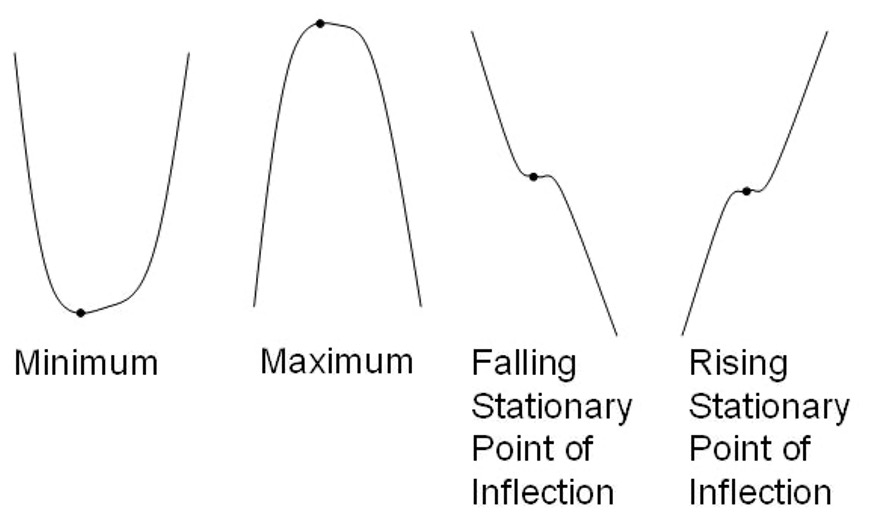
\includegraphics[width=0.5\linewidth]{Figures/Section2/212_stat_points.jpg}
    \caption{Sketch of the four types of stationary point.}
    \label{fig:stat_points}
\end{figure}

\textbf{The first derivative test.} To use this test to classify a stationary point at $x=x_0$, 
\begin{enumerate}
    \item evaluate $f'(x)$ at two points either side of $x_0$, \emph{i.e.} $f'(x_0-h)$ and $f'(x_0+h)$ for small $h$. Make sure $h$ is small enough so that $x_0 \pm h$ does not cross any other stationary points.
    \item Drawing the line \textbackslash for a negative value, / for a positive value and -- for the stationary point itself, sketch how the function looks around the stationary point (\textit{e.g.} a minimum will be \textbackslash -- /, and a maximum  / --\textbackslash).
\end{enumerate}

\textbf{The second derivative test.} To use this test to classify a stationary point at $x=x_0$, evaluate the second derivative $f''(x)$ at $x=x_0$.
\begin{itemize}
    \item If $f''(x_0) > 0$, the point is a minimum.
    \item If $f''(x_0) < 0$, the point is a maximum.
    \item If $f''(x_0) = 0$, the test is inconclusive. Fall back on the first derivative test. 
\end{itemize}

\goodbreak
\begin{example}[Lecture]
Find any stationary points for the function
\[
f(x)=2x^3-9x^2+5 \, .
\]
Use the first derivative test to classify them as maxima, minima or points of inflection. Check this using the second derivative test.
\end{example}
%
\begin{solution}
Find the first derivative
\[
f'(x)=\blank{6x^2-18x}.
\]
Solve for $f'(x)=0$.
Stationary points are at
\[
x=\blank{0}\qquad \text{and} \qquad x=\blank{3}.
\]
First derivative test for $x=0$:\par
\vspace{4mm}
\begin{tabular}{|p{10mm}|p{10mm}|p{10mm}|p{10mm}|}\hline
    $x$ & -1 & 0 & 1\\\hline
    $f'(x)$ & \blankpar{24} & 0 & \blankpar{-12}\\\hline
    sketch & \blankpar{/} & -- & \blankpar{\textbackslash}\\\hline
\end{tabular}

\vspace{4mm}
First derivative test for $x=3$:\par
\vspace{4mm}
\begin{tabular}{|p{10mm}|p{10mm}|p{10mm}|p{10mm}|}\hline
    $x$ & 2 & 3 & 4\\\hline
    $f'(x)$ & \blankpar{-12} & 0 & \blankpar{24}\\\hline
    sketch & \blankpar{\textbackslash} & -- & \blankpar{/}\\\hline
\end{tabular}
\vspace{4mm}

Find the second derivative:
\[
f''(x)=\blank{12x-18}.
\]
\[
f''(0)=\blank{-18},\qquad f''(3)=\blank{18}.
\]
Hence $x=\blank{0}$ is a \blankpar{maximum} and $x=\blank{3}$ is a \blankpar{minimum}.
\end{solution}

\subsubsection{Maximum and minimum values over an interval}

Consider the function $f(x)$ in figure \ref{fig:minmax}(a); where is the maximum? Where is the minimum? We can see there are stationary points at $a$ (\textbf{local} maximum) and $b$ (\textbf{local} minimum), but these are not the greatest or smallest values of $f(x)$ over the interval shown. In fact, the minimum over the interval shown is at the left boundary, and the maximum at the boundary. 

\begin{figure}[h!]
    \centering
    \subfig{0.8}{./Figures/Section2/213_minmax.png}{A function with local minima/maxima and greatest/least values labelled.}
    \hfill
    \subfig{0.6}{./Figures/Section2/213_point_types.jpg}{Sketch showing the different candidate points for the greatest/least values of a function in an interval.}
    \caption{}
    \label{fig:minmax}
\end{figure}

The greatest/least values of a function within an interval can occur at the following points (labelled on figure \ref{fig:minmax}(b))
\begin{enumerate}[label=(\Alph*)]
    \item Stationary points (local maxima/minima),
    \item Ends of the interval for $x$,
    \item Where $f(x)$ becomes infinite for finite $x$,
    \item Where $f(x)$ or $f'(x)$ does not exist,
    \item As $x$ becomes infinite (positive or negative).
\end{enumerate}
Such points are often referred to as \textbf{critical points}. It is a case of checking all such points in the interval. 

\goodbreak
\begin{example}[Lecture]
Find the maximum and minimum values of the function
\[
p(x)=2x^3-3x^2-36x+13
\]
on the interval $-4\leq x\leq6$.
\end{example}
%
\begin{solution}
Find first derivative
\[
p'(x)=\blank{6x^2-6x-36}.
\]
Solve for $p'(x)=0$.
\begin{align*}
    \blank{6(x^2-x-6)}&=0\\
    \blank{(x-3)(x+2)}&=0
\end{align*}
Stationary points are at $x=\blank{-2}$ and $x=\blank{3}$.

Values at stationary points:
\[
p(\blank{-2})=\blank{57},\qquad p(\blank{3})=\blank{-68}.
\]
The function $p(x)$ is continuous and finite and the bounds are finite. So just need to check the edges of the domain:
\[
p(-4)=\blank{-19},\qquad p(6)=\blank{121}.
\]
Maximum value of $\blank{121}$ at $x=\blank{6}$. Minimum value of $\blank{-68}$ at $x=\blank{3}$.
\end{solution}

\goodbreak
\begin{example}[Video]
A bioreactor produces biomass at a rate of roughly
\[
b(\omega)=3+\omega \quad [\mathrm{kg/h}],
\]
which increases with the stirring rate $\omega\geq0$ $[\mathrm{rpm}]$.
The cost of running the reactor also increases with $\omega$, roughly given by
\[
c(\omega)=72+\frac{1}{3}\omega^2 \quad [\text{\pounds}/\mathrm{h}].
\]
Find the stirring rate that optimises production efficiency (i.e. kg of biomass per \pounds$\;$spent), and the associated production efficiency.
\textbf{Note:} This can be completed once we have covered the quotient rule in section \ref{sec:quotient}).
\end{example}
%
\begin{solution}
The production efficiency (in kg of biomass per \pounds$\;$spent) is given by
\[
f(\omega)=\blank{\frac{b(\omega)}{c(\omega)}}=\blank{\frac{3+\omega}{72+\frac{1}{3}\omega^2}}.
\]
The optimal efficiency will be achieved when $f(\omega)$ is a maximum. Find the stationary points $f'(\omega)=0$, using the quotient rule:
\[
f'(\omega)=\blank{\frac{\left(72+\frac{1}{3}\omega^2\right)-(3+\omega)\frac{2}{3}\omega}{\left(72+\frac{1}{3}\omega^2\right)^2}}=0.
\]
\[
\blank{72+\frac{1}{3}\omega^2-2\omega-\frac{2}{3}\omega^2}=0.
\]
Rearranging there is a stationary point when
\[
\blank{\omega^2+6\omega-216=0}.
\]
Factorising (or using the quadratic equation)
\[
\blank{(\omega+18)(\omega-12)=0}.
\]
Since $\omega\geq0$, we have an optimal stirring rate of $\omega=\blank{12}$ $[\mathrm{rpm}]$.
Substituting this back into the equation for $f$, we get a production efficiency of
\[
f=\blank{\frac{3+12}{72+144/3}=\frac{15}{120}=\frac{1}{8}}\quad [\mathrm{kg}/\text{\pounds}].
\]
We can check this is indeed the maximum over the domain by checking $f(\omega=0) = \blank{\frac{1}{24}}$ and also $\lim_{\omega\to\infty}f(\omega) = \blank{0}$ are both \blankpar{less than} the value at the stationary point.
\end{solution}

\begin{recap}{\ref{sec:min_max}}
\item The \textbf{derivative} of a function is its gradient with respect to its variable.
\item \textbf{Local stationary points} can be found by solving $f'(x)=0$.
\item A stationary point $x_0$ is a \textbf{maximum} if $f''(x_0)<0$ and \textbf{minimum} if $f''(x_0)>0$.
\item If $f''(x_0)=0$, use the \textbf{first derivative test} instead.
\item The max and min over an interval \textbf{might not be stationary points}.
\end{recap}

\goodbreak
\subsection{The product, quotient and chain rules}
\label{sec:prod_quo_chain}

\begin{learningoutcomes}
\item Identify when to use the chain, product, or quotient rules
\item Calculate the derivatives of functions using the chain, product, or quotient rules, where appropriate
\end{learningoutcomes}

\subsubsection{The chain rule}

Consider the function
\[
f(x)=(\sin x)^2.
\]
This is a combination of two functions i.e. start with $x$, take the sine and then square it.
\[
x \quad \xrightarrow{\text{Take the sine}} \quad \sin x
\quad \xrightarrow{\text{Square it}} \quad (\sin x)^2.
\]
The inner function is $g(x)=\sin x$ and the outer function is
$h(u)=u^2$.

The chain rule tells us how to differentiate a function of a function. If $f(x)=h(u)$ where $u=g(x)$,
\begin{equation}
\label{eq:chain}  \der{f}{x} = \der{h}{u} \cdot \der{g}{x}\, ,
\end{equation}
or in alternative notation
\[
    f'(x)=h'(u)g'(x) \, ,
\]
\textit{i.e.} differentiate the outer function and multiply by the derivative of the inner function.

For the function $f(x)=(\sin x)^2$, the inner function is $u=g(x)=\sin x$. The outer function is $h(u)=u^2$. Using equation \eqref{eq:chain},
\[
f'(x)=h'(u)g'(x)=2u\cos x.
\]
Expressing in terms of $x$,
\[
f'(x)=2\sin x\cos x.
\]

\goodbreak
\begin{example}[DIY]
\label{ex:chain}
Differentiate
\[
p(t)=(t^2+1)^3
\]
using the chain rule.
\end{example}
%
\begin{blanksol}
\[
p'(t)=6t(t^2+1)^2.
\]
Let $f(t)=t^2+1$, then $p(t)=f(t)^3$. The derivative of $f(t)$ is $f'(t)=2t$. Using the chain rule
\[
p'(t)=3f'(t)f(t)^2=6t(t^2+1)^2.
\]
\end{blanksol}

Compare the solution in example \ref{ex:chain} to the result by expanding the brackets
\begin{align*}
p(t)&=(t^2+1)^3\\
&=(t^4+2t^2+1)(t^2+1)\\
&=t^6+3t^4+3t^2+1
\end{align*}
then, taking the derivative
\begin{align*}
p'(t)&=6t^5+12t^3+6t\\
&=6t(t^4+2t^2+1)\\
&=6t(t^2+1)^2.
\end{align*}
Compare this to your solution to example \ref{ex:chain}, did you get the same result? Clearly, the chain rule is more efficient. 

\textbf{Repeated chain rule.} Note the chain rule can be applied repeatedly. Consider,
\[
q(x)=e^{\sin(x^2+3)}.
\]
Write $p(x)=\sin(x^2+3)$ so that $q(x)=\exp[p(x)]$. Then, using the chain rule 
\[
q'(x)=p'(x)\exp[p(x)]
\]. 
To find $p'(x)$ use the chain rule again. Let $f(x)=x^2+3$ so $f'(x)=2x$. Then 
\[
p'(x)=f'(x)\cos f(x) \, ,
\]
and so $p'(x)=2x\cos(x^2+3)$. Using the expression for $q'(x)$ we get
\[
q'(x)=2x\cos(x^2+3)e^{\sin(x^2+3)}\, .
\]

\goodbreak
\begin{example}[Video]
\begin{enumerate}[label=(\alph*)]
    \item Find the derivative of
            \[
            y=e^{3(1-g^2(x))}
            \]
    in terms of the unknown function $g(x)$ and its derivative $g'(x)$.
    \item When $g(x)=\cos x$, what is $y'$?
\end{enumerate}
\end{example}
%
\begin{solution}
(a) First define
\[
h(x)=\blank{3(1-g^2)=3-3g^2},
\]
then
\[
h'(x)=\blank{-6gg'}.
\]
And so
\[
\blank{y'=h'e^h=-6gg'e^{3(1-g^2)}}.
\]

(b) If $g(x)=\cos x$ then $g'(x)=\blank{-\sin x}$ and therefore
\begin{align*}
y'&=\blank{-6gg'e^{3(1-g^2)}}\\
&=\blank{6\sin x\cos x\,e^{3(1-\cos^2x)}}\\
&=\blank{6\sin x\cos x\,e^{3\sin^2x}}.
\end{align*}
\end{solution}

\textbf{The Chain Rule and Linear Functions.} Consider the following functions and how to differentiate them.
\[
f(x)=\sin\left(4x+\frac{\pi}{2}\right)
\]
\[
g(x)=5e^{2x-9}
\]
\[
h(x)=7\ln(6-2x)
\]
\[
p(x)=(7x+9)^{10}.
\]

Each of these functions can be differentiated using the chain rule \textit{e.g.}
\[
f(x)=\sin\left(4x+\frac{\pi}{2}\right)
\]
\[
f'(x)=\cos\left(4x+\frac{\pi}{2}\right)\times4
\]
\[
=4\cos\left(4x+\frac{\pi}{2}\right).
\]

Each of these functions is of the form
\[
f(ax+b)
\]
and has derivative
\[
af'(ax+b).
\]

\goodbreak
\begin{example}[Lecture]
Differentiate
\[
r(x)=2\cos(5x-\pi)
\]
and
\[
p(x)=\ln(2x+1).
\]
\end{example}
%
\begin{solution}
\[
r'(x)=\blank{-10\sin(5x-\pi)}.
\]
\[
p'(x)=\blank{\frac{2}{2x+1}}.
\]
\end{solution}

\subsubsection{The product rule}

Consider the function
\[
f(x)=x\sin x.
\]
This is a product of two functions $u(x)=x$ and $v(x)=\sin x$. The product rule enables the differentiation of a product of two functions.

If
\[
f(x)=u(x)v(x),
\]
then the \textbf{product rule} states
\begin{equation}
    \der{}{x}(uv)=v\frac{{\rm d}u}{{\rm d}x}+u\frac{{\rm d}v}{{\rm d}x}.
\end{equation}

or, in alternative notation
\[
f'(x)=u'(x)v(x)+u(x)v'(x),
\]
\emph{i.e.} multiply each function by the derivative of the other and add together. Note, it \textbf{does not matter} which function is $u$ and which function is $v$.

In the case $f(x)=x\sin x$, let $u(x)=x$ and $v(x)=\sin x$. Then $u'(x)=1$ and $v'(x)=\cos x$. Using $f'(x)=uv'+vu'$,
\[
f'(x)=x\cos x+\sin x.
\]

\goodbreak
\begin{example}[Lecture]
Differentiate
\[
g(x)=3x^2\ln x
\]
using the product rule.
\end{example}
%
\begin{solution}
Let $u(x)=\blank{3x^2}$ and $v(x)=\blank{\ln x}$. Then $u'(x)=\blank{6x}$ and $v'(x)=\blank{1/x}$. Using the product rule $g'(x)=uv'+u'v$,
\[
g'(x)=\blank{3x+6x\ln x}=\blank{3x(1+2\ln x)}.
\]
\end{solution}

\textbf{The product rule for products of three or more functions.} Consider
\[
f(x)=u(x)v(x)w(x)
\]
and make the substitution
\[
s(x)=v(x)w(x)
\]
so that
\[
f(x)=u(x)s(x).
\]

Thus
\[
f'(x)=u's+us'\, .
\]
Using the product rule for $s(x)=v(x)w(x)$:
\[
s'(x)=v'w+vw'\,.
\]
Substituting into $f'(x)$:
\begin{align}
f'(x)&=u'vw+u(v'w+vw')\\
&=u'vw+uv'w+uvw'
\end{align}
gives the sum of three terms. Each is the product of two functions multiplied by the derivative of the third function.

\goodbreak
\begin{example}[Video]
Differentiate
\[
g(x)=x^2e^x\sin(\pi x)
\]
using the product rule.
\end{example}
%
\begin{solution}
Define $u(x)=x^2$, $v(x)=e^x$, and $w(x)=\sin(\pi x)$, so that $g=uvw$.

The product rule for three functions states that
\[
g'=u'vw+uv'w+uvw'.
\]
Find the derivatives of $u$, $v$, and $w$:
\[
u'=\blank{2x},
\qquad
v'=\blank{e^x},
\qquad
w'=\blank{\pi\cos(\pi x)}.
\]
And substitute them into the expression for $g'$:
\[
\blank{g'=2xe^x\sin(\pi x)
+x^2e^x\sin(\pi x)
+x^2e^x\pi\cos(\pi x)}.
\]
Which can be factorised as
\[
\blank{g'=xe^x\left[2\sin(\pi x)+x\sin(\pi x)+\pi x\cos(\pi x)\right]}
\]
\[
\blank{=xe^x\left[(x+2)\sin(\pi x)+\pi x\cos(\pi x)\right]}.
\]
\end{solution}

\subsubsection{The quotient rule}
\label{sec:quotient}

Consider the function
\[
f(x)=\frac{\sin x}{x}.
\]
This is a quotient of two functions \textit{i.e.} one function divided by another. The quotient rule enables the differentiation of a quotient of two functions.

If
\[
f(x)=\frac{u(x)}{v(x)},
\]
then the quotient rule states
\begin{equation}
    \der{}{x}\left(\frac{u}{v}\right)
= \frac{v\dfrac{{\rm d}u}{{\rm d}x}-u\dfrac{{\rm d}v}{{\rm d}x}}{v^2} \, .
\end{equation}
or in alternative notation
\[
f'(x)=\frac{u'v-uv'}{v^2}.
\]
Unlike the product rule, it is now \textbf{critical} which is $u$ and which is $v$.

\goodbreak
\begin{example}[Lecture]
Differentiate
\[
g(x)=\frac{\ln x}{x^2}
\]
by two methods:
\begin{enumerate}
\item[(a)] Using the quotient rule
\item[(b)] Writing as $g(x)=x^{-2}\ln x$ and using the product rule.
\end{enumerate}
\end{example}
%
\begin{solution}
(a) Let $u(x)=\ln x$ and $v(x)=x^2$. Then
\[
u'(x)=\blank{\frac{1}{x}}
\qquad\text{and}\qquad
v'(x)=\blank{2x}.
\]
Using the quotient rule
\[
g'(x)=\frac{u'v-uv'}{v^2}=\blank{\frac{x-2x\ln x}{x^4}}
\]
\[
=\frac{1-2\ln x}{x^3}.
\]

(b) Now let $u(x)=\ln x$ and $v(x)=x^{-2}$. Then
\[
u'(x)=\blank{\frac{1}{x}}
\qquad\text{and}\qquad
v'(x)=\blank{-2x^{-3}}.
\]
Using the product rule
\[
g'(x)=u'v+uv'=\blank{\frac{1}{x}x^{-2}-2x^{-3}\ln x}
\]
\[
=\blank{\frac{1-2\log x}{x^3}}.
\]
\end{solution}

\goodbreak
\begin{example}[Video]
Differentiate $x$ with respect to $t$, where
\[
x=\frac{e^{2t}\sin(t^3)}{t}.
\]
\end{example}
%
\begin{solution}
Define $u(t)=e^{2t}\sin(t^3)$ and $v(t)=t$ and find their derivatives.

For $u'(t)$, we need to use the product rule and chain rule:
\begin{align*}
u'(t)&=\blank{2e^{2t}\sin(t^3)+e^{2t}3t^2\cos(t^3)}\\
&=\blank{e^{2t}\left[2\sin(t^3)+3t^2\cos(t^3)\right]}.
\end{align*}
and
\[
v'(t)=\blank{1}\, .
\]
The quotient rule states
\[
x'=\frac{u'v-v'u}{v^2}.
\]
Substituting in the expressions for $u$, $v$, $u'$, and $v'$ gives
\begin{align*}
x'&=\blank{\frac{e^{2t}\left[2\sin(t^3)+3t^2\cos(t^3)\right]t-e^{2t}\sin(t^3)}{t^2}}\\
&=\blank{e^{2t}\left[\frac{2t-1}{t^2}\sin(t^3)+3t\cos(t^3)\right]}\,.
\end{align*}
\end{solution}

\begin{recap}{\ref{sec:prod_quo_chain}}
\item The \textbf{chain rule}: if $f(x)=h(u)$ where $u=g(x)$ then
\[
f'(x)=h'(u)g'(x).
\]
\item The \textbf{product rule}: if $f(x)=u(x)v(x)$ then
\[
f'(x)=u'v+uv'.
\]
\item The \textbf{quotient rule}: If $f(x)=u(x)/v(x)$ then
\[
f'(x)=\frac{u'v-uv'}{v^2}.
\]
\end{recap}

\goodbreak
\subsection{Implicit, logarithmic, and parametric differentiation}
\label{sec:other_diff_rules}

\begin{learningoutcomes}
\item Identify when to use implicit, logarithmic, and parametric differentiation
\item Calculate the derivatives of functions using implicit, logarithmic, and parametric differentiation, where appropriate
\end{learningoutcomes}

\subsubsection{Implicit differentiation}

Consider the implicit relation
\[
x^2+y^2=25.
\]
Although written in implicit form, it can be differentiated. It is important to know which variable we are differentiating with respect to. In this case, we want to find ${\rm d}y/{\rm d}x$.

Differentiate term-by-term with respect to $x$:
\begin{itemize}
\item The derivative of $x^2$ is $2x$
\item Using the chain rule, the derivative of $y^2$ is $2y\der{y}{x}$
\item The derivative of 25 is zero
\end{itemize}
Therefore, we have
\[
2x+2y\der{y}{x}=0.
\]
Which rearranges to
\[
\der{y}{x}=-\frac{x}{y}.
\]
This is an example of \textbf{implicit differentiation}.

The second derivative can also be found by repeating the process. Starting with $x^2+y^2=25$ and differentiating we get
\[
2x+2y\der{y}{x}=0.
\]
\begin{itemize}
\item Differentiating $2x$ gives 2
\item Using the product rule, differentiating $2y\der{y}{x}$ gives $2\left(\der{y}{x}\right)^2+2y\der{^2y}{x^2}$
\end{itemize}
So, we find
\[
2+2\left(\der{y}{x}\right)^2+2y\der{^2y}{x^2}=0
\]
or
\[
\der{^2y}{x^2}=-\frac{1+\left(\der{y}{x}\right)^2}{y}.
\]
Substituting in the result from before (${\rm d}y/{\rm d}x=-x/y$), this reduces to
\[
\der{^2y}{x^2}=-\frac{1}{y}-\frac{x^2}{y^3}.
\]

Alternatively, we could start with the result for ${\rm d}y/{\rm d}x$, \emph{i.e.}
\[
\der{y}{x}=-\frac{x}{y}.
\]
Use the quotient rule to differentiate, with $u=-x$ and $v=y$, so $u'=-1$ and $v'=y'$:
\[
\der{^2y}{x^2}=\frac{u'v-v'u}{v^2}=\frac{-y+xy'}{y^2}.
\]
Substituting in the previous result $y'=-x/y$ gives
\[
\der{^2y}{x^2}=\frac{-y-x^2/y}{y^2}=-\frac{1}{y}-\frac{x^2}{y^3},
\]
\emph{i.e.} the same result as before.

\goodbreak
\begin{example}[Lecture]
If
\[
x^4+2xy+y^4=1,
\]
find the derivatives ${\rm d}y/{\rm d}x$ and $d^2y/{\rm d}x^2$ at the point $x=1$, $y=0$.
\end{example}
%
\begin{solution}
Differentiate the equation with respect to $x$ and rearrange for ${\rm d}y/{\rm d}x$.
\begin{align*}
\blank{4x^3 + 2y + 2x\der{y}{x} + 4y^3\der{y}{x}}&=\blank{0}\\
\blank{(4y^3+2x)\der{y}{x}} &= \blank{-(4x^3 + 2y)}\\
\der{y}{x}&=\blank{-\frac{4x^3+2y}{2x+4y^3}}
\end{align*}
Differentiate the original expression again and rearrange for $d^2y/{\rm d}x^2$.
\begin{align*}
\blank{12x^2 + 4\der{y}{x} + 2x\der{^2y}{x^2} + 12y^2\left(\der{y}{x}\right)^2 + 4y^3\der{^2y}{x^2}} = \blank{0}\\
\blank{(2x+4y^3)\der{^2y}{x^2}} = \blank{-12y^2\left(\der{y}{x}\right)^2 - 4\der{y}{x} - 12x^2}\\
\therefore \; \der{^2y}{x^2}=\blank{-\frac{12x^2+4y'+12y^2(y')^2}{2x+4y^3}}.
\end{align*}
At $x=1$ and $y=0$,
\[
\der{y}{x}=\blank{-\frac{4\times 1^3}{2\times 1}} = \blank{-2}
\]
Using this in the expression for the second derivative, we find that at $x=1$ and $y=0$,
\[
\der{^2y}{x^2}=\blank{-\frac{12\times1^2+ 4\times(-2)}{2\times 1}} = \blank{-2}\,.
\]
\end{solution}

\subsubsection{Logarithmic differentiation}

Logarithmic differentiation is a special case of implicit differentiation. It can make derivatives simpler by taking advantage of the properties of logarithms, such as
\begin{itemize}
\item Transforming products into sums: $\ln(ab)=\ln a+\ln b$
\item Transforming powers into coefficients: $\ln(x^n)=n\ln x$
\end{itemize}

E.g. consider a function of the form
\[
y=f(x)g(x)h(x).
\]
On taking the logarithm of the absolute value of both sides,
\[
\ln |y|=\ln|fgh|
\]
\[
=\ln| f|+\ln |g|+\ln |h|.
\]
Using implicit differentiation, the derivative of the left-hand side is
\[
\der{}{x}(\ln |y|)=\frac{1}{y}\der{y}{x}.
\]
Differentiating both sides and using this rule gives
\[
\frac{1}{y}\der{y}{x}=\frac{f'}{f}+\frac{g'}{g}+\frac{h'}{h}.
\]

Therefore, using logarithmic differentiation
\[
y=f(x)g(x)h(x)
\]
gives
\[
\der{y}{x}=y\left(\frac{f'(x)}{f(x)}+\frac{g'(x)}{g(x)}+\frac{h'(x)}{h(x)}\right).
\]
This could have also been arrived at by rearranging the product rule for three functions.

\goodbreak
\begin{example}[Lecture]
Use logarithmic differentiation to find the derivative of
\[
y=\frac{\sqrt{(x+a)(x+b)}}{x-c}.
\]
\end{example}
%
\begin{solution}
Take natural log of the absolute value of both sides:
\[
\ln |y|=\ln\left|\frac{\sqrt{(x+a)(x+b)}}{x-c}\right|.
\]
Use the product log rule:
\[
\ln |y|=\blank{\ln\sqrt{x+a}+\ln\sqrt{x+b}-\ln|x-c|}.
\]
Use power log rule:
\[
\ln |y|=\blank{\frac{1}{2}\ln|x+a|+\frac{1}{2}\ln|x+b|-\ln|x-c|}.
\]
Differentiate both sides with respect to $x$:
\[
\frac{1}{y}\der{y}{x}=\blank{\frac{1}{2(x+a)}+\frac{1}{2(x+b)}-\frac{1}{x-c}}.
\]
Rearrange and substitute in expression for $y$:
\[
\der{y}{x}=\blank{\frac{\sqrt{(x+a)(x+b)}}{x-c}\left(\frac{1}{2(x+a)}+\frac{1}{2(x+b)}-\frac{1}{x-c}\right)}.
\]
\end{solution}

\goodbreak
\begin{example}[Video]
Find the derivative, with respect to $t$, of
\[
z=3^{t^2-1}.
\]
\end{example}
%
\begin{solution}
Take the natural logarithm (note $z > 0$) of both sides to give
\[
\ln z = \blank{\ln\left|3^{t^2-1}\right|=(t^2-1)\ln(3)}.
\]
Differentiate both sides with respect to $t$:
\[
\frac{z'}{z}=\blank{2t\ln3}.
\]
Rearrange and substitute back in the expression for $z$ to get
\[
z'=\blank{2t\ln3\,z=2t\ln3\,3^{t^2-1}}.
\]
Alternatively, you could rearrange to write as
\[
z=\blank{e^{\ln(3)(t^2-1)}}
\]
and differentiate using the chain rule.
\end{solution}

\subsubsection{Parametric differentiation}

A parametric function can also be differentiated. Consider the parametric function
\[
y=f(t) \qquad x=g(t).
\]
The derivative of $y$ with respect to $x$ is given by
\begin{equation}
    \der{y}{x}=\frac{{\rm d}y/{\rm d}t}{{\rm d}x/{\rm d}t}=\frac{f'(t)}{g'(t)}
\end{equation}


Consider, for example,
\[
y=\sin t \qquad x=\cos t,
\]
\emph{i.e.} the unit circle. Here
\[
\der{y}{x}=\frac{{\rm d}y/{\rm d}t}{{\rm d}x/{\rm d}t}=\frac{\cos t}{-\sin t}=-\cot t.
\]
The animation in figure \ref{anim:parametric_diff} demonstrates this by adding the tangent line to the parametric form of the unit circle (as used in figure \ref{anim:parametric}). Projecting to the $x$-$t$ plane, the tangent line has gradient ${\rm d}x/{\rm d}t$, for the $y$-$t$ plane it is ${\rm d}y/{\rm d}t$ and so as we project to the $x$-$y$ plane the tangent has gradient $\frac{{\rm d}y/{\rm d}t}{{\rm d}x/{\rm d}t}=\der{y}{x}$. This is visualised by the relationship between the components of the tangent line in figure \ref{fig:tangent_project}

\begin{figure}[h!]
    \iflatexml
            \<div id="parametric-curve-widget-with-tangent" data-r="1">\</div> 
            \<script src="https://cdn.plot.ly/plotly-3.0.1.min.js">\</script>
            \<script src="bmluser/parametric-curve-widget-with-tangent.js">\</script>
        \caption{Interactive plot of the parametric curve $x=\cos t$, $y=\sin t$, as shown in figure \ref{anim:parametric}. The tangent line in black shows the gradient at the highlighted point.}
    \else
    \centering
    \subfig{0.33}{Figures/Section2/parametric_curve_widget_diff_xt.png}{$x-t$ plane}
    \hfill
    \subfig{0.33}{Figures/Section2/parametric_curve_widget_diff_yt.png}{$y-t$ plane}
    \hfill
    \subfig{0.25}{Figures/Section2/parametric_curve_widget_diff_xy.png}{$x-y$ plane}
    \caption{Screenshots of the interactive plot of the parametric curve $x=\cos t$, $y=\sin t$, available in the html version of these notes. The tangent line in black shows the gradient at the highlighted point. }
    \fi
    \label{anim:parametric_diff}
\end{figure}

\begin{figure}[ht]
    \centering
    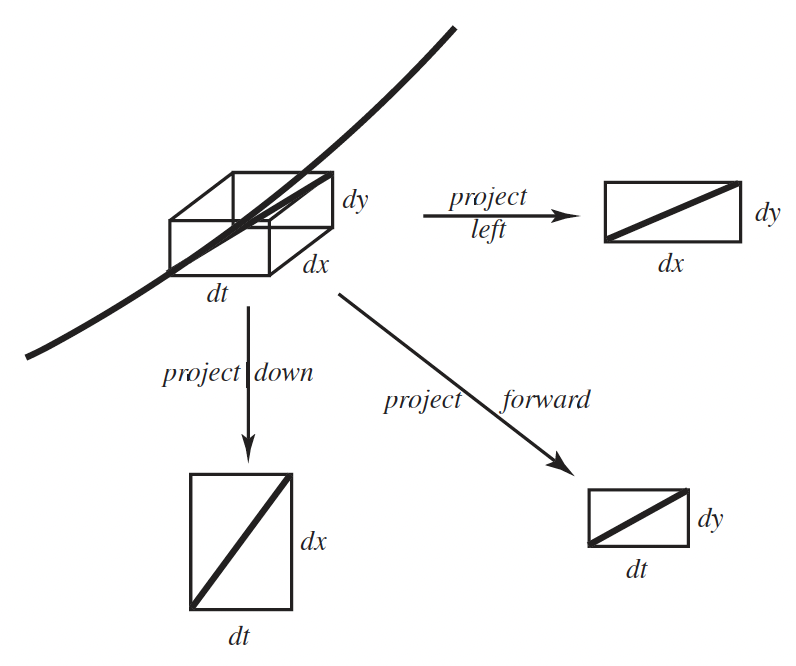
\includegraphics[width=0.6\linewidth]{Figures/Section2/233_parametric_diff.png}
    \caption{We can think of the tangent line as the ratio of the components of the derivatives ${\rm d}x$, ${\rm d}y$, and ${\rm d}t$, and so the relation $\der{y}{x}=\frac{{\rm d}y/{\rm d}t}{{\rm d}x/{\rm d}t}$ follows from simple geometry. (Figure from Tall 2013 ``\textit{How Humans Learn to Think Mathematically}'', Chapter 11).}
    \label{fig:tangent_project}
\end{figure}


The process can be extended to the second derivative (and higher order derivatives). Define
\[
z(t)=\der{y}{x},
\]
then repeat the process to find the derivative of $z$ with respect to $x$:
\[
\der{^2y}{x^2}=\frac{dz}{{\rm d}x}=\frac{dz/{\rm d}t}{{\rm d}x/{\rm d}t}.
\]

Continuing the previous example,
\[
y=\sin t \qquad x=\cos t \qquad \der{y}{x}=-\cot t.
\]
Now
\[
\der{^2y}{x^2}=\frac{dz}{{\rm d}x}=\frac{dz/{\rm d}t}{{\rm d}x/{\rm d}t}
\]
\[
=\frac{d(-\cot t)/{\rm d}t}{-\sin t}=\frac{\csc^2t}{-\sin t}=-\frac{1}{\sin^3t}
\]
\[
=-\frac{1}{y^3}.
\]
Note it is not always convenient to express the derivative in terms of $x$ and $y$.

\newtexpage
\begin{exammistake}
Using
\[
\der{^2y}{x^2}=\frac{d^2y/{\rm d}t^2}{d^2x/{\rm d}t^2}
\]
instead of
\[
\der{^2y}{x^2}=\frac{dz/{\rm d}t}{{\rm d}x/{\rm d}t}, \qquad \text{where} \qquad z=\der{y}{x}.
\]

\begin{quote}
\textbf{25/26 Exam Q2(a)(i).} The equations
\[
x=\sin\left(\frac{\pi t}{6}\right)
\qquad\text{and}\qquad
y=t^2-3t+3
\]
describe a curve in parametric form. Find expressions for ${\rm d}y/{\rm d}x$ and $d^2y/{\rm d}x^2$ in terms of t.
\end{quote}

\textbf{Correct answer:}
\[
\der{^2y}{x^2}
=
\frac{6\left[12\cos\left(\frac{\pi t}{6}\right)+(2t-3)\pi\sin\left(\frac{\pi t}{6}\right)\right]}
{\pi^2\cos^3\left(\frac{\pi t}{6}\right)}. \qquad \checkmark
\]

\textbf{Using the incorrect definition}
\[
\frac{d^2y/{\rm d}t^2}{d^2x/{\rm d}t^2}=-\frac{72}{\pi^2\sin\left(\frac{\pi t}{6}\right)}. \qquad \text{\sffamily X}
\]
\end{exammistake}

\goodbreak
\begin{example}[Lecture]
Find the derivative ${\rm d}y/{\rm d}x$ and the second derivative $d^2y/{\rm d}x^2$ given that
\[
x=t^3+t \qquad y=e^{2t}.
\]
\end{example}
%
\begin{solution}
Find derivatives of $x$ and $y$:
\[
\der{x}{t}=\blank{3t^2+1}
\qquad
\der{y}{t}=\blank{2e^{2t}}.
\]
Take the ratio:
\[
\der{y}{x}=\frac{{\rm d}y/{\rm d}t}{{\rm d}x/{\rm d}t}=\blank{\frac{2e^{2t}}{3t^2+1}}.
\]
Use quotient rule for $dz/{\rm d}t$:
\[
u(t)=\blank{2e^{2t}}
\qquad\text{and}\qquad
v(t)=\blank{3t^2+1}.
\]
Find the derivatives:
\[
u'(t)=\blank{4e^{2t}}
\qquad\text{and}\qquad
v'(t)=\blank{6t}.
\]
Substitute in:
\[
\frac{dz}{{\rm d}t}=\frac{u'v-uv'}{v^2}
=\blank{\frac{4e^{2t}(3t^2+1)-12te^{2t}}{(3t^2+1)^2}}.
\]
and therefore
\[
\der{^2y}{x^2}=\frac{dz/{\rm d}t}{{\rm d}x/{\rm d}t}
=\blank{\frac{4(3t^2-3t+1)}{(3t^2+1)^3}e^{2t}}.
\]
\end{solution}

\begin{recap}{\ref{sec:other_diff_rules}}
    \item \textbf{Implicit differentiation} is performed by differentiating each term in an equation of the form $f(x,y)=0$ with respect to $x$ and rearranging for ${\rm d}y/{\rm d}x$.
    \item \textbf{Logarithmic differentiation} of a function $y=g(x)$ involves taking the log of both sides first to simplify the RHS:
    \[
    \frac{1}{y}\der{y}{x}=\der{}{x}\ln(g(x)).
    \]
    \item To find ${\rm d}y/{\rm d}x$ when $x$ and $y$ are in \textbf{parametric form}, use the relationship
    \[
    \der{y}{x}=\frac{{\rm d}y/{\rm d}t}{{\rm d}x/{\rm d}t}.
    \]
\end{recap}
